\documentclass[10pt,a4paper]{article}

\usepackage[latin1]{inputenc}
\usepackage{amsmath}
\usepackage{amsfonts}
\usepackage{amssymb}
\usepackage{graphicx}
\usepackage{listings}

\begin{document}

\title{Answer to reviewers \\
jFuzzyLogic: A Robust and Flexible Fuzzy-Logic Inference System Language Implementation
}
\author{Pablo Cingolani and Jes\'us Alcal\'a-Fdez}

\date{}
\maketitle

\section{REVIEW NO. 1}

Comments to the authors:

   This work is definitely related to the topics of the session on "Software for
   Soft Computing". It presents jFuzzyLogic, an open source library for making
   easier the design of fuzzy controllers. The manuscript is well-written and
   organized. I only have some minor comments and suggestions aimed to improve even
   more the quality of the present work:

\begin{itemize}

   \item[1)] In section II, authors claim "a comparison of freely available fuzzy logic
   software" but what about commercial software?

	\item[\textbf{Answer}] We clarified in the main text that it is no the intention of this paper to perform a comprehensive comparison of all available fuzzy logic packages. We limited the comparison 
	to freely available packages since this is the category were jFuzzyLogic belongs 
	as well as the most commonly used in academic environments.

   \item[2)] Even though the paper focuses on fuzzy control, please notice that there are
   some free software tools (that should be taken into account in this work) for
   fuzzy modeling which offer advances methods for generation of fuzzy systems no
   matter the specific application domain where they will be used. Look at tools
   like Xfuzzy (http://www2.imse-cnm.csic.es/Xfuzzy/), Fispro
   (http://www.inra.fr/mia/M/fispro/FisPro\_EN.html), GUAJE
   (http://www.softcomputing.es/guaje), etc. Obviously, partitions and rules
   designed with such tools may be later translated into the FCL format and being
   used with jFuzzyLogic.

	\item[\textbf{Answer}] The suggested software packages have been added to our comparison table. 
	We agree that software developers should embrace the use of standards instead of trying to define their own formats. 
	jFuzzyLogic, provides a library with a ready to use implementation of the standard, thus alleviating much of the work for all developers.

   \item[3)] You should remark, someway, on Table I those five software packages that
   "seemed to be maintained, compiled correctly, and had extensive functionality",
   putting special emphasis on those two which are based on jFuzzyLogic.

	\item[\textbf{Answer}] As suggested, we added an asterisk after the package name (e.g. jFuzzyLogic$^\ast$) to indicate that that package ``seems to be maintained, compiles correctly, and has extensive functionality". The packages based on jFuzzyLogic were marked as 'Uses jFuzzyLogic' in the notes column.

   \item[4)] Table I includes information about the number of membership functions (MF),
   but what about their type/shape?

	\item[\textbf{Answer}] We clarified in the main text that the most common membership functions is trapezoid and it's special cases (triangular, rectangular, etc.). 
	Nevertheless, as we pointed out before, it is not the intention to perform a comprehensive review of the all avalaible packages. So, for the sake of brevity, we don't enumerate all membership functions for all packages.
		
   \item[5)] Be careful, Table II (page 4) should turn up before Table III (page 3). In
   addition, check the use of quotation marks in Table III.

	\item[\textbf{Answer}] As suggested, we corrected the listing style to show quotes properly as well as the table order.

   \item[6)] Are tables II to V formal tables? In fact, they are listing code. You should
   use verbatim package or something similar.

	\item[\textbf{Answer}] We are using package ``listings''. We added \textit{basicstyle=\\ttfamily} to \textit{lsset} command in order to make it similar to verbatim package.
	
   \item[7)] You should plot the fuzzy partitions related to the example detailed in
   Tables II and III. It would help to understand better the example making it much
   more illustrative. Moreover, the rule base defined is made up of only three
   rules and as a result it is incomplete, i.e., it does not cover all possible
   situations. What is the suggested tip in case service=1 and food=4 (in the
   current example none of the three rules would be fired)?

	\item[\textbf{Answer}] i-) As suggested, we added a figure showing the membership functions for that example.

	ii-) The rule base is not incomplete. In case service = 1 and food = 4, rule 
	number 1 is activated ("if service is poor OR ...").

   \item[8)] The notation used in Tables II, IV and V are not exactly the same. For
   instance, Table II does not include DEFAULT related to DEFUZZIFY. AND/ACT/ACCU
   are also missing in the RULEBLOCK. This fact should be corrected or explicitely
   noted in the paper.
   
   	\item[\textbf{Answer}] 
   	i-) By no means this paper is intended to be an FCL handbook or a resurce to learn the language. FCL is only briefly introduced and some examples are shown just to show how easy to learn the language is. Nevertheless, we repeatedly refer to the FCL specification (IEC-61131-7) for those who are interested in learning the details of the language.

   	ii-) In FCL, the mentioned statements (DEFUZZIFY, ACT and ACCU) are optional and have sensitive defaults. Thus all these statements can be omitted. Showing that they can be omitted is also part of the examples.

   \item[9)] In Section III.C authors state that "a few optimization algorithms are
   already implemented... other optimization algorithms can be implemented". Coming
   back to what I say in 2) there are many algorithms useful for fuzzy modeling
   that may be directly applicable in the context of jFuzzyLogic. The only thing
   missing is the right parser to translate from one format to other.

	\item[\textbf{Answer}] We do agree that the main problem is that each software developer creates custom formats. 
	Obviously jFuzzyLogic is intended to help alleviate this problem by providing a common ground implementation of the standard that developers can use. 
	This greatly simplifies the work to software developers who want to adopt the standard.
	
	Of course, using a standard means that there is no longer need for 'translating from one format to the other'. 
	Thus saving time on irrelevant tasks.

   \item[10)] In Fig.3, be sure that variable names are in accordance with Table IV, but
   also with the related explanation in Section IV (page 5).

   	\item[\textbf{Answer}] Variable names have been changed accordingly.

   \item[11)] In "Acknowledgement" use the full names of authors instead of PC and JAF.
   
   	\item[\textbf{Answer}] The names have been changed accordingly.
   	


   \item[12)] Some minor typos:

\begin{itemize}
   \item[12.1)] "Figure" should be substituted by "Fig." according to WCCI templates.

   \item[12.2)] "of a [the] wall following" (page5)

   \item[12.3)] "The [main] requirement[s] ... is[are]..." (page5)

   \item[12.4)] "More than one output variable[s]" (page5)

   \item[12.5)] Check the use of quotation marks all along the paper.

   \item[12.6)] Ref2. pages?

   \item[12.7)] Ref5. "An introduction[industrial] reality"

   \item[12.8)] Ref10. C.J. Cabrera J.A. ?

   \item[12.9)] Ref11. I.E.C.?
\end{itemize}

   \item[\textbf{Answer}] All changes have been incorporated.

\end{itemize}



\section{REVIEW NO. 2}

Comments to the authors:
   The paper presents a library for designing fuzzy logic controllers. The library
   is called jFuzzyLogic. It is written in Java and respects the FCL (fuzzy control
   language) IEC-61131-7 specifications. FCL is an instruction list oriented
   programming language.
   The aim is to provide a standardized language and parser, which could be
   interesting for designing industrial fuzzy controllers.

   The paper is clear and easy to read.

    However some points are questionable.
    
\begin{itemize}   
   \item[1)] The state of the art of fuzzy logic software given in the introduction is
   incomplete and does not include fuzzy software such as Xfuzzy, FisPro,
   Guaje, Nefclass... It should absolutely be completed to avoid giving
   false information to the readers.

   \item[\textbf{Answer}] See answer to item 1 from reviewer 1.
   
   \item[2)] Another flaw is the use of misleading terms in Part IIIB. What the authors
   call aggregation is usually called combination in rule premises.
   Similarly, activation is in fact the result of an implication operator.
   Activation should not be confused with rule matching degree.
    Here again, accumulation is usually called rule aggregation.

   \item[\textbf{Answer}] We added the following sentence to clarify this:
   
\textit{It should be noted that we adhere to the definitions of Aggregation, Activation and Accumulation as defined by IEC-61131-7, which may differ from the naming conventions from other references (e.g. ``Aggregation" may sometimes be called ``Combination").}
   
   The reviewer points out another way to call these methods/operators. 
   Since this paper focuses on IEC implementation, we prefer stick to the definitions provided by the norm. 
   The norm clearly defines terms and how they are used. 
   Moreover the operator in FCL is called 'ACCU' not 'AGGR', so changing the terminology as proposed would be extremely confusing. 
   We refer the reviewer IEC-61131-7 pages 71 to 77 for details of these definitions. 
   We reproduce here figure A.2.3. for his convince.
   
\begin{figure}[!h]
\centering
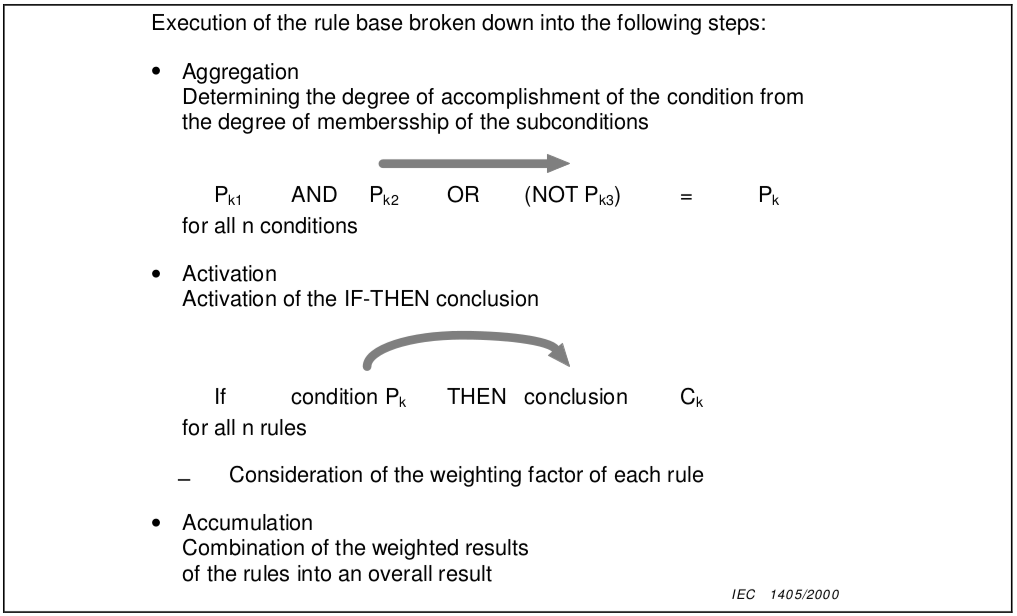
\includegraphics[width=5in]{figs/AccAgg.png}
\caption{Aggregation, Activation and Accumulation as defines in IEC-61131-7.}
\label{f:tipperMf}
\end{figure}

    
   \item[3)] Part IIIb mentions that the membership functions (MFs) are systematically
   discretized. It seems a pity for analytical forms very easy to compute such as
   trapezoidal or triangular MFs.
   
   \item[\textbf{Answer}] It is true that we sacrifice performance in order to be able to have generic membership functions.
   This is because jFuzzyLogic is very flexible and accepts arbitrarily defined functions.

   We are thinking on implementing such performance optimization in future releases of our software. 
   Specially when the fuzzy system is simple and only includes trapezoidal membership functions.
   
\end{itemize}

    The paper quality  would be improved if the authors could address the following
   two topics:

\begin{itemize}   
   \item[1)] hierarchical controllers.
   How is one block linked to another one?
   
   \item[\textbf{Answer}] This can be done using the java API. It was clarified in the main text.
   
   \item[2)] optimization.
   Is the specification of the data used for optimizing
   the membership functions included in the FLC model?

   \item[\textbf{Answer}] The norm only defines FCL language. Optimization is implemented as an additional feature in our package.

   \item[3)] English spelling and grammar: could be improved.
   for instance: page2, these limitation -> these limitations
   page 4, non neglible -> non-neglectable
   page 5, gradient descend -> gradient descent
   page 5, a the wall -> the wall
   case of study -> case study

	\item[\textbf{Answer}] We corrected the text as suggested.
	
\end{itemize}

\section{REVIEW NO. 3}

Comments to the authors:

\begin{itemize}  
   \item The paper is acceptable, but I would be happier if it had stronger evaluation
   section.
   
   	\item[\textbf{Answer}] As suggested by this and the other reviewers, we added some packages to the comparison table.
   	
 \end{itemize}
   

\end{document}
